\documentclass[10pt,a4paper]{article}
\usepackage[top=1.4cm, bottom=1.4cm, left=1.6cm, right=1.6cm, headheight=14pt, footskip=18pt]{geometry}
\usepackage[utf8]{inputenc}
\usepackage{amsmath,amsfonts,amssymb}
\usepackage{graphicx}
\usepackage{tikz}
\usepackage{circuitikz}
\usetikzlibrary{calc,patterns}
\usepackage[most]{tcolorbox}
\usepackage{enumitem}
\usepackage{fancyhdr}
\usepackage{booktabs}
\usepackage{tabularx}
\usepackage{colortbl}
\usepackage{hyperref}

% --- Palet Warna Resmi UNIB ---
\definecolor{unibblue}{RGB}{0, 32, 96}
\definecolor{unibgold}{RGB}{197, 160, 89}
\definecolor{unibgreen}{RGB}{34, 112, 60}
\definecolor{boxbg}{RGB}{248, 250, 253}
\definecolor{linegray}{RGB}{210, 215, 225}

% --- Pengaturan Header & Footer ---
\pagestyle{fancy}
\fancyhf{}
\lhead{\footnotesize\textbf{\color{unibblue}Universitas Bengkulu} \textbar\ Program Studi S1 Teknik Elektro}
\rhead{\footnotesize\color{gray}Persamaan Diferensial (Genap 2026)}
\lfoot{\footnotesize\color{gray}Problem Set Tugas Terstruktur Berbasis OBE}
\cfoot{\footnotesize\color{gray}Hal. \thepage\ dari 2}
\rfoot{\footnotesize\color{unibblue}\textbf{Minggu 13: Persamaan Laplace \& Medan Potens...}}
\renewcommand{\headrulewidth}{0.6pt}
\renewcommand{\footrulewidth}{0.4pt}

\begin{document}

% ==================== HALAMAN 1 ====================
\noindent\begin{minipage}[c]{0.68\textwidth}%
  {\large\textbf{\color{unibblue}PROBLEM SET (TUGAS MANDIRI TERSTRUKTUR)}}\\[1mm]
  {\normalsize\textbf{Mata Kuliah: Persamaan Diferensial (2 SKS)}}\\[0.5mm]
  {\small\textbf{Topik Minggu 13:} Persamaan Laplace \& Medan Potensial Elektrostatika 2D}%
\end{minipage}%
\hfill%
\begin{minipage}[c]{0.30\textwidth}%
  \begin{tcolorbox}[colback=unibblue!5,colframe=unibblue,boxrule=0.6pt,arc=2pt,left=4pt,right=4pt,top=2pt,bottom=2pt]
    \scriptsize
    \textbf{Nama:} \dotfill\\[1.2mm]
    \textbf{NPM:} \dotfill\\[1.2mm]
    \textbf{Kelas/Klp:} \dotfill\\[1.2mm]
    \textbf{Nilai Final:} \hfill \textbf{/ 100}
  \end{tcolorbox}%
\end{minipage}\par

\vspace{1.5mm}

% Kotak Sub-CPMK & Pedoman Tugas Terstruktur
\begin{tcolorbox}[colback=boxbg,colframe=unibgold!90!black,boxrule=0.6pt,arc=2pt,left=5pt,right=5pt,top=3pt,bottom=3pt,title=\textbf{\scriptsize Capaian Pembelajaran (Sub-CPMK 6) \& Pedoman Pengerjaan Tugas}]
  \scriptsize
  \textbf{Sub-CPMK 6:} Mahasiswa mampu menyelesaikan Persamaan Laplace 2D (PDP Eliptik) dengan metode pemisahan variabel koordinat Kartesian untuk menentukan distribusi potensial dan medan listrik pada geometri elektroda isolator.\\
  \textbf{Ketentuan Tugas:} Kerjakan secara mandiri pada kertas folio/A4 bergaris atau laporan digital rapi. Lampirkan penurunan rumus analitis lengkap dan cetak visualisasi kode program Julia (Soal C6). Kumpulkan pada awal perkuliahan minggu berikutnya.
\end{tcolorbox}

\vspace{1.5mm}

\noindent{\textbf{\color{unibblue}\large BAGIAN I: FONDASI KONSEPTUAL \& PENURUNAN MATEMATIS}}\par
\vspace{1mm}

% Soal C1
\noindent\textbf{1. (C1 - Mengingat \textbar\ Bobot: 10 Poin)}\par\vspace{0.8mm}
{\footnotesize Tuliskan bentuk Persamaan Diferensial Parsial Laplace $\nabla^2 V = 0$ dalam koordinat Kartesian 2D $\frac{\partial^2 V}{\partial x^2} + \frac{\partial^2 V}{\partial y^2} = 0$, dan sebutkan perbedaan fisis antara Persamaan Laplace (ruang bebas muatan) dan Persamaan Poisson (ruang bermuatan).}\par

\vspace{2.5mm}

% Soal C2
\noindent\textbf{2. (C2 - Memahami \textbar\ Bobot: 15 Poin)}\par\vspace{0.8mm}
{\footnotesize Jelaskan prinsip fisis di balik Teorema Nilai Rata-Rata (*Mean Value Theorem*) untuk medan harmonik: mengapa nilai potensial listrik di sembarang titik selalu sama dengan rata-rata potensial pada permukaan bola/lingkaran yang melingkupinya, dan mengapa titik ekstremum lokal hanya dapat terjadi pada batas (*boundary*)?}\par

\vspace{2.5mm}

% Soal C3
\noindent\textbf{3. (C3 - Menerapkan \textbar\ Bobot: 20 Poin)}\par\vspace{0.8mm}
\noindent\begin{minipage}[t]{0.60\textwidth}%
  {\footnotesize Tinjau alur celah isolator tegangan tinggi berdimensi persegi panjang semi-tak-hingga ($0 \le x \le a, y \ge 0$) pada gambar di samping. Batas samping dan bawah dibumikan ($V(0,y) = 0, V(a,y) = 0, V(x,\infty) = 0$), sedangkan batas pelat atas dipertahankan pada tegangan konstan $V(x,0) = V_0$. Gunakan pemisahan variabel untuk menurunkan fungsi potensial $V(x,y)$!}%
\end{minipage}%
\hfill%
\begin{minipage}[t]{0.37\textwidth}%
  \centering
  \resizebox{0.95\linewidth}{!}{%
  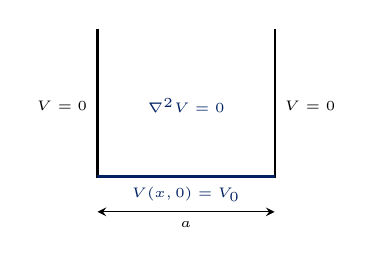
\begin{tikzpicture}[scale=0.75]
    \draw[thick] (0,2.5) -- (0,0) -- (3.0,0) -- (3.0,2.5);
    \draw[thick, unibblue] (0,0) -- (3.0,0) node[midway, below, font=\tiny\bfseries] {$V(x,0)=V_0$};
    \node at (-0.6,1.2) [font=\tiny] {$V=0$};
    \node at (3.6,1.2) [font=\tiny] {$V=0$};
    \node at (1.5,1.2) [font=\tiny, unibblue] {$\nabla^2 V = 0$};
    \draw[<->, >=stealth] (0,-0.6) -- (3.0,-0.6) node[midway, below, font=\tiny] {$a$};
  \end{tikzpicture}%
  }%
\end{minipage}\par

\vfill

% Kotak Formula Rujukan Teknis & Standar Industri
\begin{tcolorbox}[colback=unibblue!3,colframe=unibblue,colbacktitle=unibblue,coltitle=white,boxrule=0.6pt,arc=2pt,left=6pt,right=6pt,top=3pt,bottom=3pt,title=\textbf{\scriptsize FORMULA RUJUKAN TEKNIS \& STANDAR INDUSTRI TERKAIT}]
  \scriptsize
  \begin{itemize}[leftmargin=*, nosep]
  \item Persamaan Laplace Elektrostatika Bebas Muatan ($\rho_v = 0$): $\nabla^2 V = \frac{\partial^2 V}{\partial x^2} + \frac{\partial^2 V}{\partial y^2} = 0$
  \item Hubungan Medan Listrik dan Potensial Skalar: $\vec{E} = -\nabla V = -\left(\frac{\partial V}{\partial x}\hat{a}_x + \frac{\partial V}{\partial y}\hat{a}_y\right)$
  \item Metode Pemisahan Variabel (*Separation of Variables*): $V(x,y) = X(x) Y(y)$
  \item Kekuatan Dielektrik Udara (Tegangan Tembus Udara Kering): $E_{\text{kritis}} \approx 30\text{ kV/cm} = 3\text{ MV/m}$
\end{itemize}
\end{tcolorbox}

\newpage
% ==================== HALAMAN 2 ====================

\noindent{\textbf{\color{unibblue}\large BAGIAN II: ANALISIS SISTEM, EVALUASI STANDAR, \& KOMPUTASI JULIA}}\par
\vspace{1mm}

% Soal C4
\noindent\textbf{4. (C4 - Menganalisis \textbar\ Bobot: 20 Poin)}\par\vspace{0.8mm}
{\footnotesize Berdasarkan solusi potensial $V(x,y)$ dari Soal 3: (a) Turunkan ekspresi vektor medan listrik $\vec{E}(x,y) = -\nabla V = -\left(\frac{\partial V}{\partial x}\hat{a}_x + \frac{\partial V}{\partial y}\hat{a}_y\right)$; (b) Tentukan lokasi titik terjadinya stres medan listrik maksimum $\vec{E}_{\text{maks}}$; (c) Analisis potensi terjadinya lucutan korona (*corona discharge*) jika $V_0 = 100\text{ kV}$ dan $a = 10\text{ cm}$ (kuat dielektrik udara $30\text{ kV/cm}$).}\par

\vspace{3.5mm}

% Soal C5
\noindent\textbf{5. (C5 - Mengevaluasi \textbar\ Bobot: 20 Poin)}\par\vspace{0.8mm}
{\footnotesize Evaluasi distribusi kerapatan muatan induksi permukaan $\sigma_s(x) = -\epsilon_0 \left. \frac{\partial V}{\partial y} \right|_{y=0}$ pada pelat konduktor batas. Buktikan bahwa muatan cenderung terkonsentrasi di sudut-sudut tajam elektroda (*edge effect*), dan jelaskan relevansi rekayasa penambahan cincin perata medan (*corona ring*) pada isolator gardu induk PLN.}\par

\vspace{3.5mm}

% Soal C6
\noindent\textbf{6. (C6 - Merancang \& Komputasi Julia \textbar\ Bobot: 15 Poin)}\par\vspace{0.8mm}
{\footnotesize Rancang program ilmiah berbasis \textbf{Julia} untuk menyelesaikan Persamaan Laplace 2D pada geometri Soal 3 menggunakan metode relaksasi beda hingga (FDM Jacobi / Gauss-Seidel). Program harus menghasilkan peta kontur garis ekuipotensial 2D berdampingan dengan panah medan vektor gradien $\vec{E}$.}\par

\vfill

% Tabel Rekapitulasi Skor OBE & Lembar Catatan Umpan Balik Dosen
\noindent\begin{minipage}[b]{0.62\textwidth}%
  \centering
  \scriptsize
  \begin{tabular}{|c|c|c|c|c|c|c|}
    \hline
    \rowcolor{unibblue}
    \textbf{\color{white}C1} & \textbf{\color{white}C2} & \textbf{\color{white}C3} & \textbf{\color{white}C4} & \textbf{\color{white}C5} & \textbf{\color{white}C6} & \textbf{\color{white}Total} \\
    \rowcolor{unibblue!10}
    10 Pts & 15 Pts & 20 Pts & 20 Pts & 20 Pts & 15 Pts & 100 Pts \\
    \hline
    & & & & & & \\[3mm]
    \hline
  \end{tabular}%
\end{minipage}%
\hfill%
\begin{minipage}[b]{0.35\textwidth}%
  \centering
  \scriptsize
  \textbf{Verifikasi Dosen / Asisten:}\\[6mm]
  (\dotfill)\\[1mm]
  \tiny Tanggal: \dotfill
\end{minipage}\par

\vspace{2mm}
\begin{tcolorbox}[colback=white,colframe=unibblue!40!black,colbacktitle=unibblue!10,coltitle=unibblue,boxrule=0.5pt,arc=2pt,left=5pt,right=5pt,top=3pt,bottom=3pt,title=\textbf{\tiny Catatan Evaluasi \& Umpan Balik Dosen Pengampu}]
  \tiny
  \textbf{Rubrik Pemeriksaan Pengerjaan Tugas Mandiri:}\par\vspace{0.8mm}
  $\square$ Penurunan matematis langkah-demi-langkah runtut (C1--C4) \hfill $\square$ Validasi analitis \& standar industri IEEE/IEC/SPLN akurat (C5)\\[0.8mm]
  $\square$ Skrip program Julia mandiri \& grafik visualisasi terlampir (C6) \hfill $\square$ Kerapian format laporan \& ketepatan waktu pengumpulan\\[2.0mm]
  \textbf{Catatan / Koreksi Khusus Dosen:}\\[1.6cm]
\end{tcolorbox}

\end{document}
